%%%%%%%%%%%%%%%%%%%%%%%%%%%%%%%%%%%%%%%%%
% Jacobs Landscape Poster
% LaTeX Template
% Version 1.0 (29/03/13)
%
% Created by:
% Computational Physics and Biophysics Group, Jacobs University
% https://teamwork.jacobs-university.de:8443/confluence/display/CoPandBiG/LaTeX+Poster
%
% Further modified by:
% Nathaniel Johnston (nathaniel@njohnston.ca)
%
% Modified further still by:
% Abraham Nunes (nunes <at> dal <dot> ca)
%
% License:
% CC BY-NC-SA 3.0 (http://creativecommons.org/licenses/by-nc-sa/3.0/)
%
%%%%%%%%%%%%%%%%%%%%%%%%%%%%%%%%%%%%%%%%%

%----------------------------------------------------------------------------------------
%	PACKAGES AND OTHER DOCUMENT CONFIGURATIONS
%----------------------------------------------------------------------------------------

\documentclass[final,table]{beamer}
\usepackage{multirow}
\usepackage{subcaption}

\usepackage[scale=1.24]{beamerposter} % Use the beamerposter package for laying out the poster
\usepackage{array}
\usetheme{confposter} % Use the confposter theme supplied with this template
\usepackage{bm}
\usepackage{xspace}
\usepackage{mathtools}
\usepackage{bm}
\usepackage{multirow}
\usepackage{adjustbox}
\setbeamercolor{block title}{fg=black,bg=} % Colors of the block titles
\setbeamercolor{block body}{fg=black,bg=} % Colors of the body of blocks
\setbeamercolor{block alerted title}{fg=white,bg=black} % Colors of the highlighted block titles
\setbeamercolor{block alerted body}{fg=black,bg=white} % Colors of the body of highlighted blocks
% Many more colors are available for use in beamerthemeconfposter.sty

\newcommand{\deemph}[1]{{\color{black!40}#1}}

%-----------------------------------------------------------
% Define the column widths and overall poster size
% To set effective sepwid, onecolwid and twocolwid values, first choose how many columns you want and how much separation you want between columns
% In this template, the separation width chosen is 0.024 of the paper width and a 4-column layout
% onecolwid should therefore be (1-(# of columns+1)*sepwid)/# of columns e.g. (1-(4+1)*0.024)/4 = 0.22
% Set twocolwid to be (2*onecolwid)+sepwid = 0.464
% Set threecolwid to be (3*onecolwid)+2*sepwid = 0.708

\newlength{\sepwid}
\newlength{\onecolwid}
\newlength{\twocolwid}
\newlength{\threecolwid}
\setlength{\paperwidth}{48in} % A0 width: 46.8in
\setlength{\paperheight}{36in} % A0 height: 33.1in
\setlength{\sepwid}{0.024\paperwidth} % Separation width (white space) between columns
\setlength{\onecolwid}{0.22\paperwidth} % Width of one column
\setlength{\twocolwid}{0.464\paperwidth} % Width of two columns
\setlength{\threecolwid}{0.708\paperwidth} % Width of three columns
\setlength{\topmargin}{-0.5in} % Reduce the top margin size

\makeatletter
\newcommand{\srcsize}{\@setfontsize{\srcsize}{5pt}{5pt}}
\makeatother

\setbeamerfont{bibliography entry author}{size=\tiny,}
\setbeamerfont{bibliography entry title}{size=\tiny}
\setbeamerfont{bibliography entry location}{size=\tiny,}
\setbeamerfont{bibliography entry note}{size=\tiny,}
%-----------------------------------------------------------

\usepackage{graphicx}  % Required for including images
\usepackage{amsmath} % assumes amsmath package installed
\usepackage{amssymb}  % assumes amsmath package installed
\usepackage[mathscr]{euscript}


% \usepackage{lmodern} % get rid of warnings
% \usepackage{caption} % improved spacing between figure and caption
%
% \DeclareCaptionLabelSeparator{horse}{:\quad} % change according to your needs
% \captionsetup{
%   labelsep = horse,
%   figureposition = bottom
% }
%
% \setbeamertemplate{caption}[numbered]
%
%
% % \setbeamerfont{caption}{size=\footnotesize}
% % \setbeamertemplate{caption}[numbered]
%


\usepackage{booktabs} % Top and bottom rules for tables
\usepackage{setspace}
\DeclarePairedDelimiter\abs{\lvert}{\rvert}%
\DeclarePairedDelimiter\norm{\lVert}{\rVert}%
\newcommand\Set[2]{\{\,#1\mid#2\,\}}

%----------------------------------------------------------------------------------------
%	TITLE SECTION
%----------------------------------------------------------------------------------------

\title{A Digital Framework for Fraternal Transitions in Individuality} % Poster title

\author{Matthew Andres Moreno and Charles Ofria} % Author(s)

\institute{Michigan State University}% Institution(s)

%----------------------------------------------------------------------------------------

\setbeamerfont{caption}{size=\footnotesize}
\setbeamertemplate{caption}{%
    \structure{\textbf{\insertcaptionname~\insertcaptionnumber:}}
    \raggedright\insertcaption\par
}

\begin{document}
\addtobeamertemplate{block begin}{}{\raggedright} % White space under blocks1
\addtobeamertemplate{block end}{}{\vspace*{1ex}} % White space under blocks1
\addtobeamertemplate{block alerted end}{}{\vspace*{0.5ex}} % White space under highlighted (alert) blocks

\setlength{\belowcaptionskip}{0ex} % White space under figures
\setlength\belowdisplayshortskip{2ex} % White space under equations

\begin{frame}[t] % The whole poster is enclosed in one beamer frame
\vspace{-1ex}
\begin{columns}[t] % The whole poster consists of three major columns, the second of which is split into two columns twice - the [t] option aligns each column's content to the top

\begin{column}{\sepwid}\end{column} % Empty spacer column

\begin{column}{\onecolwid} % The first column

%----------------------------------------------------------------------------------------
%	INTRODUCTION
%----------------------------------------------------------------------------------------
\begin{block}{Introduction}

\begin{alertblock}{Fraternal Transitions}
\begin{figure}
 \centering
  \begin{columns}
  \begin{column}{0.10\textwidth}
   \textbf{(a)}
  \end{column}
  \begin{column}{0.65\textwidth}
    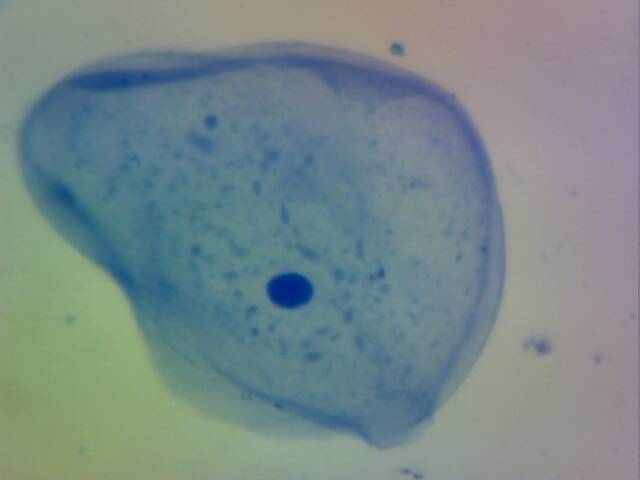
\includegraphics[width=\textwidth]{img/cheek_cell}
  \end{column}
  \begin{column}{0.05\textwidth}
    \cite{clare_and_ben_2017}
  \end{column}
  \end{columns}
  \begin{columns}
  \begin{column}{0.10\textwidth}
   \textbf{(b)}
  \end{column}
  \begin{column}{0.65\textwidth}
    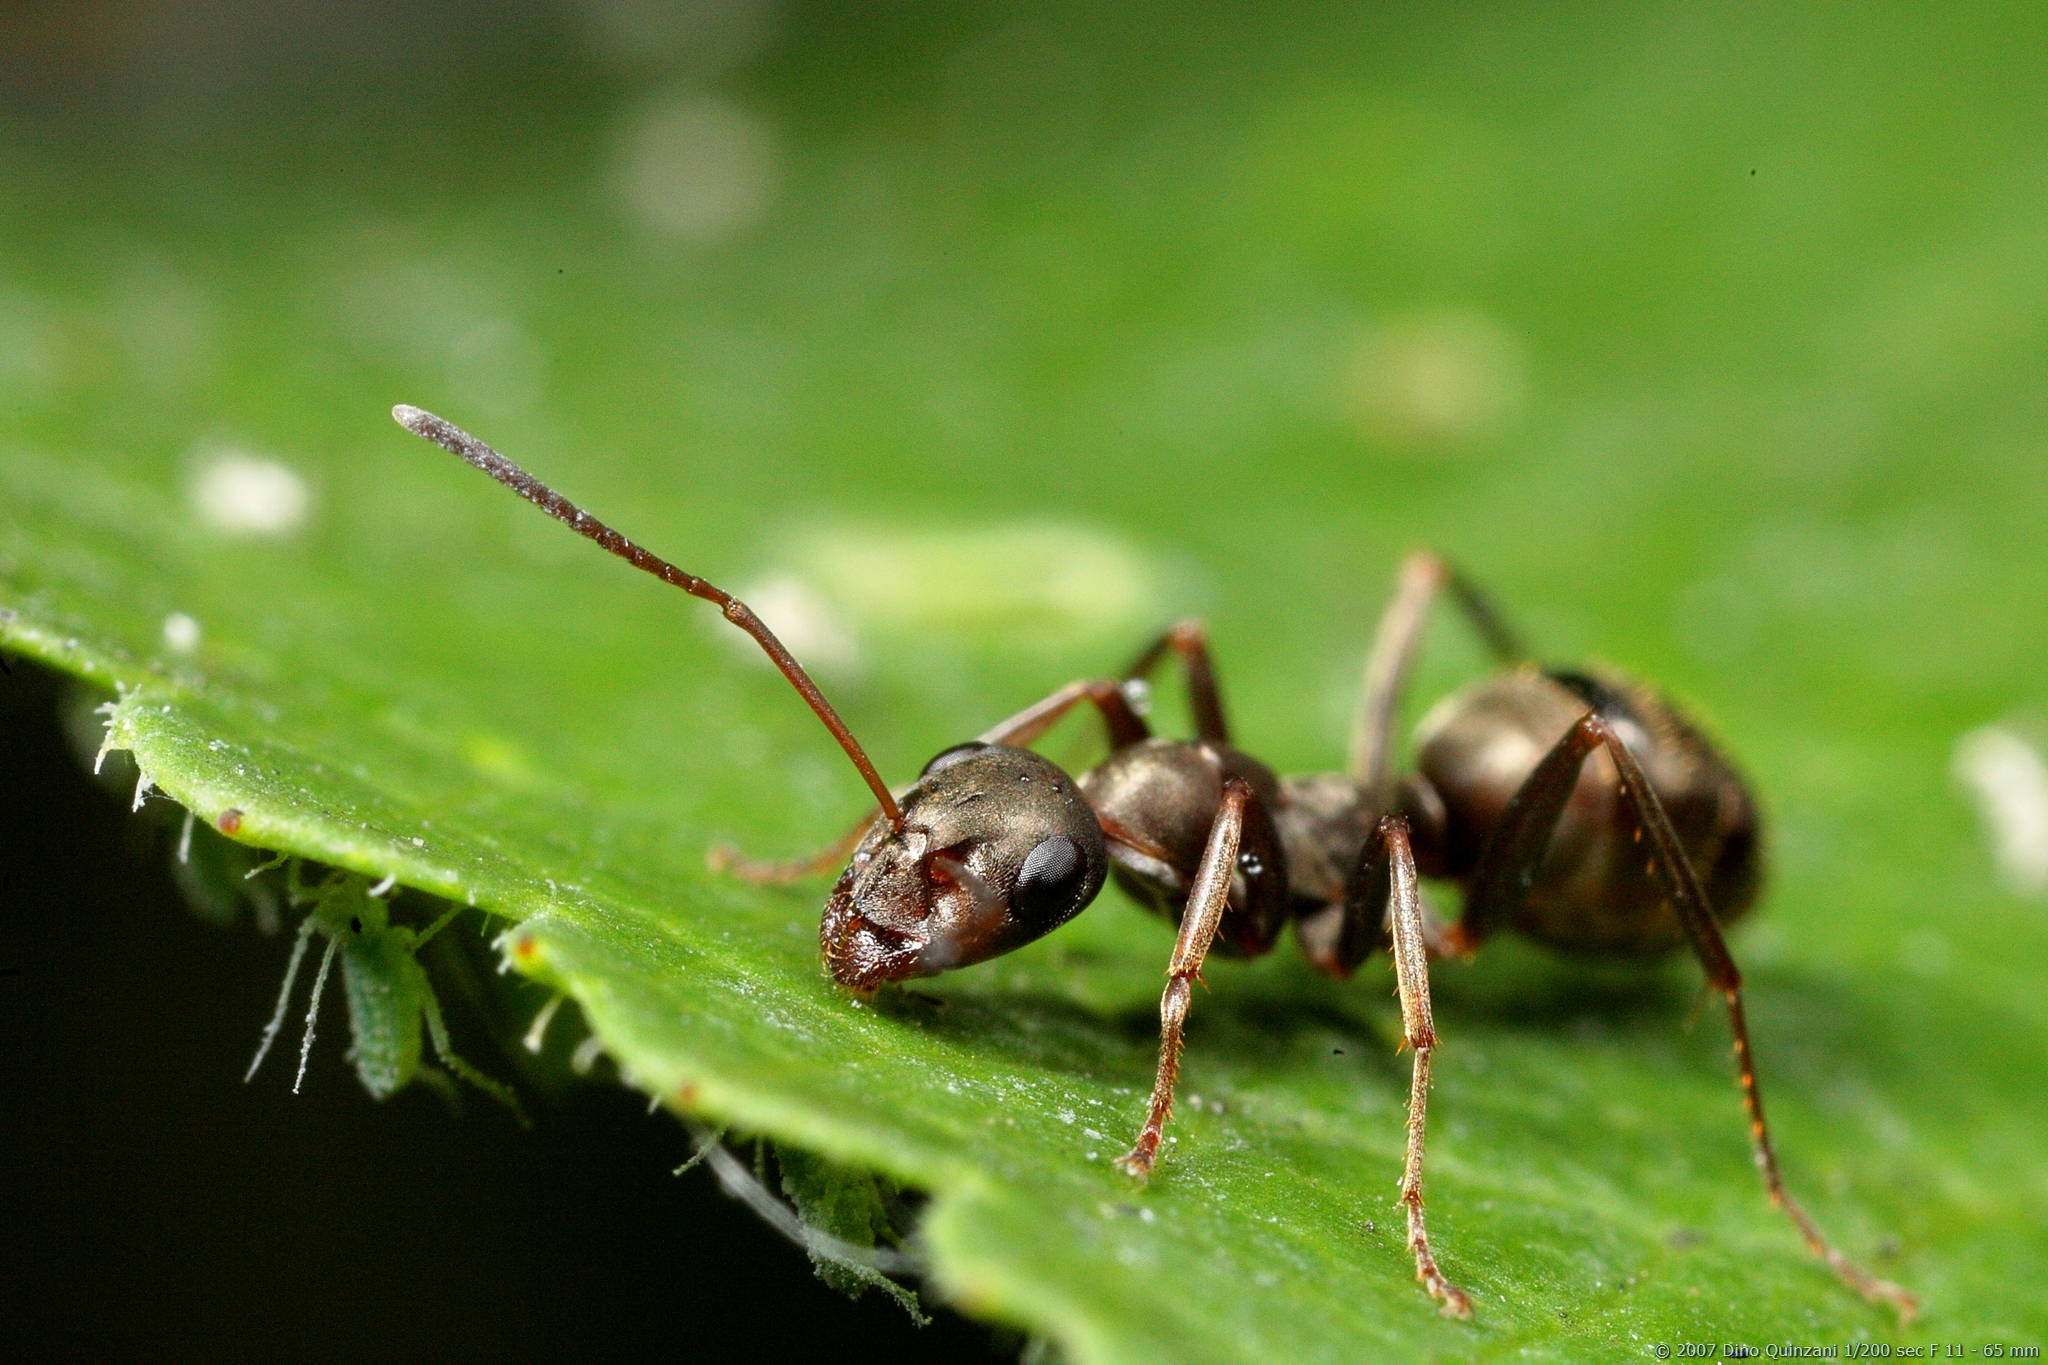
\includegraphics[width=\textwidth]{img/ant}
  \end{column}
  \begin{column}{0.05\textwidth}
    \cite{quinzani_2008}
  \end{column}
  \end{columns}
  \begin{columns}
  \begin{column}{0.10\textwidth}
    \textbf{(c)}
  \end{column}
  \begin{column}{0.65\textwidth}
    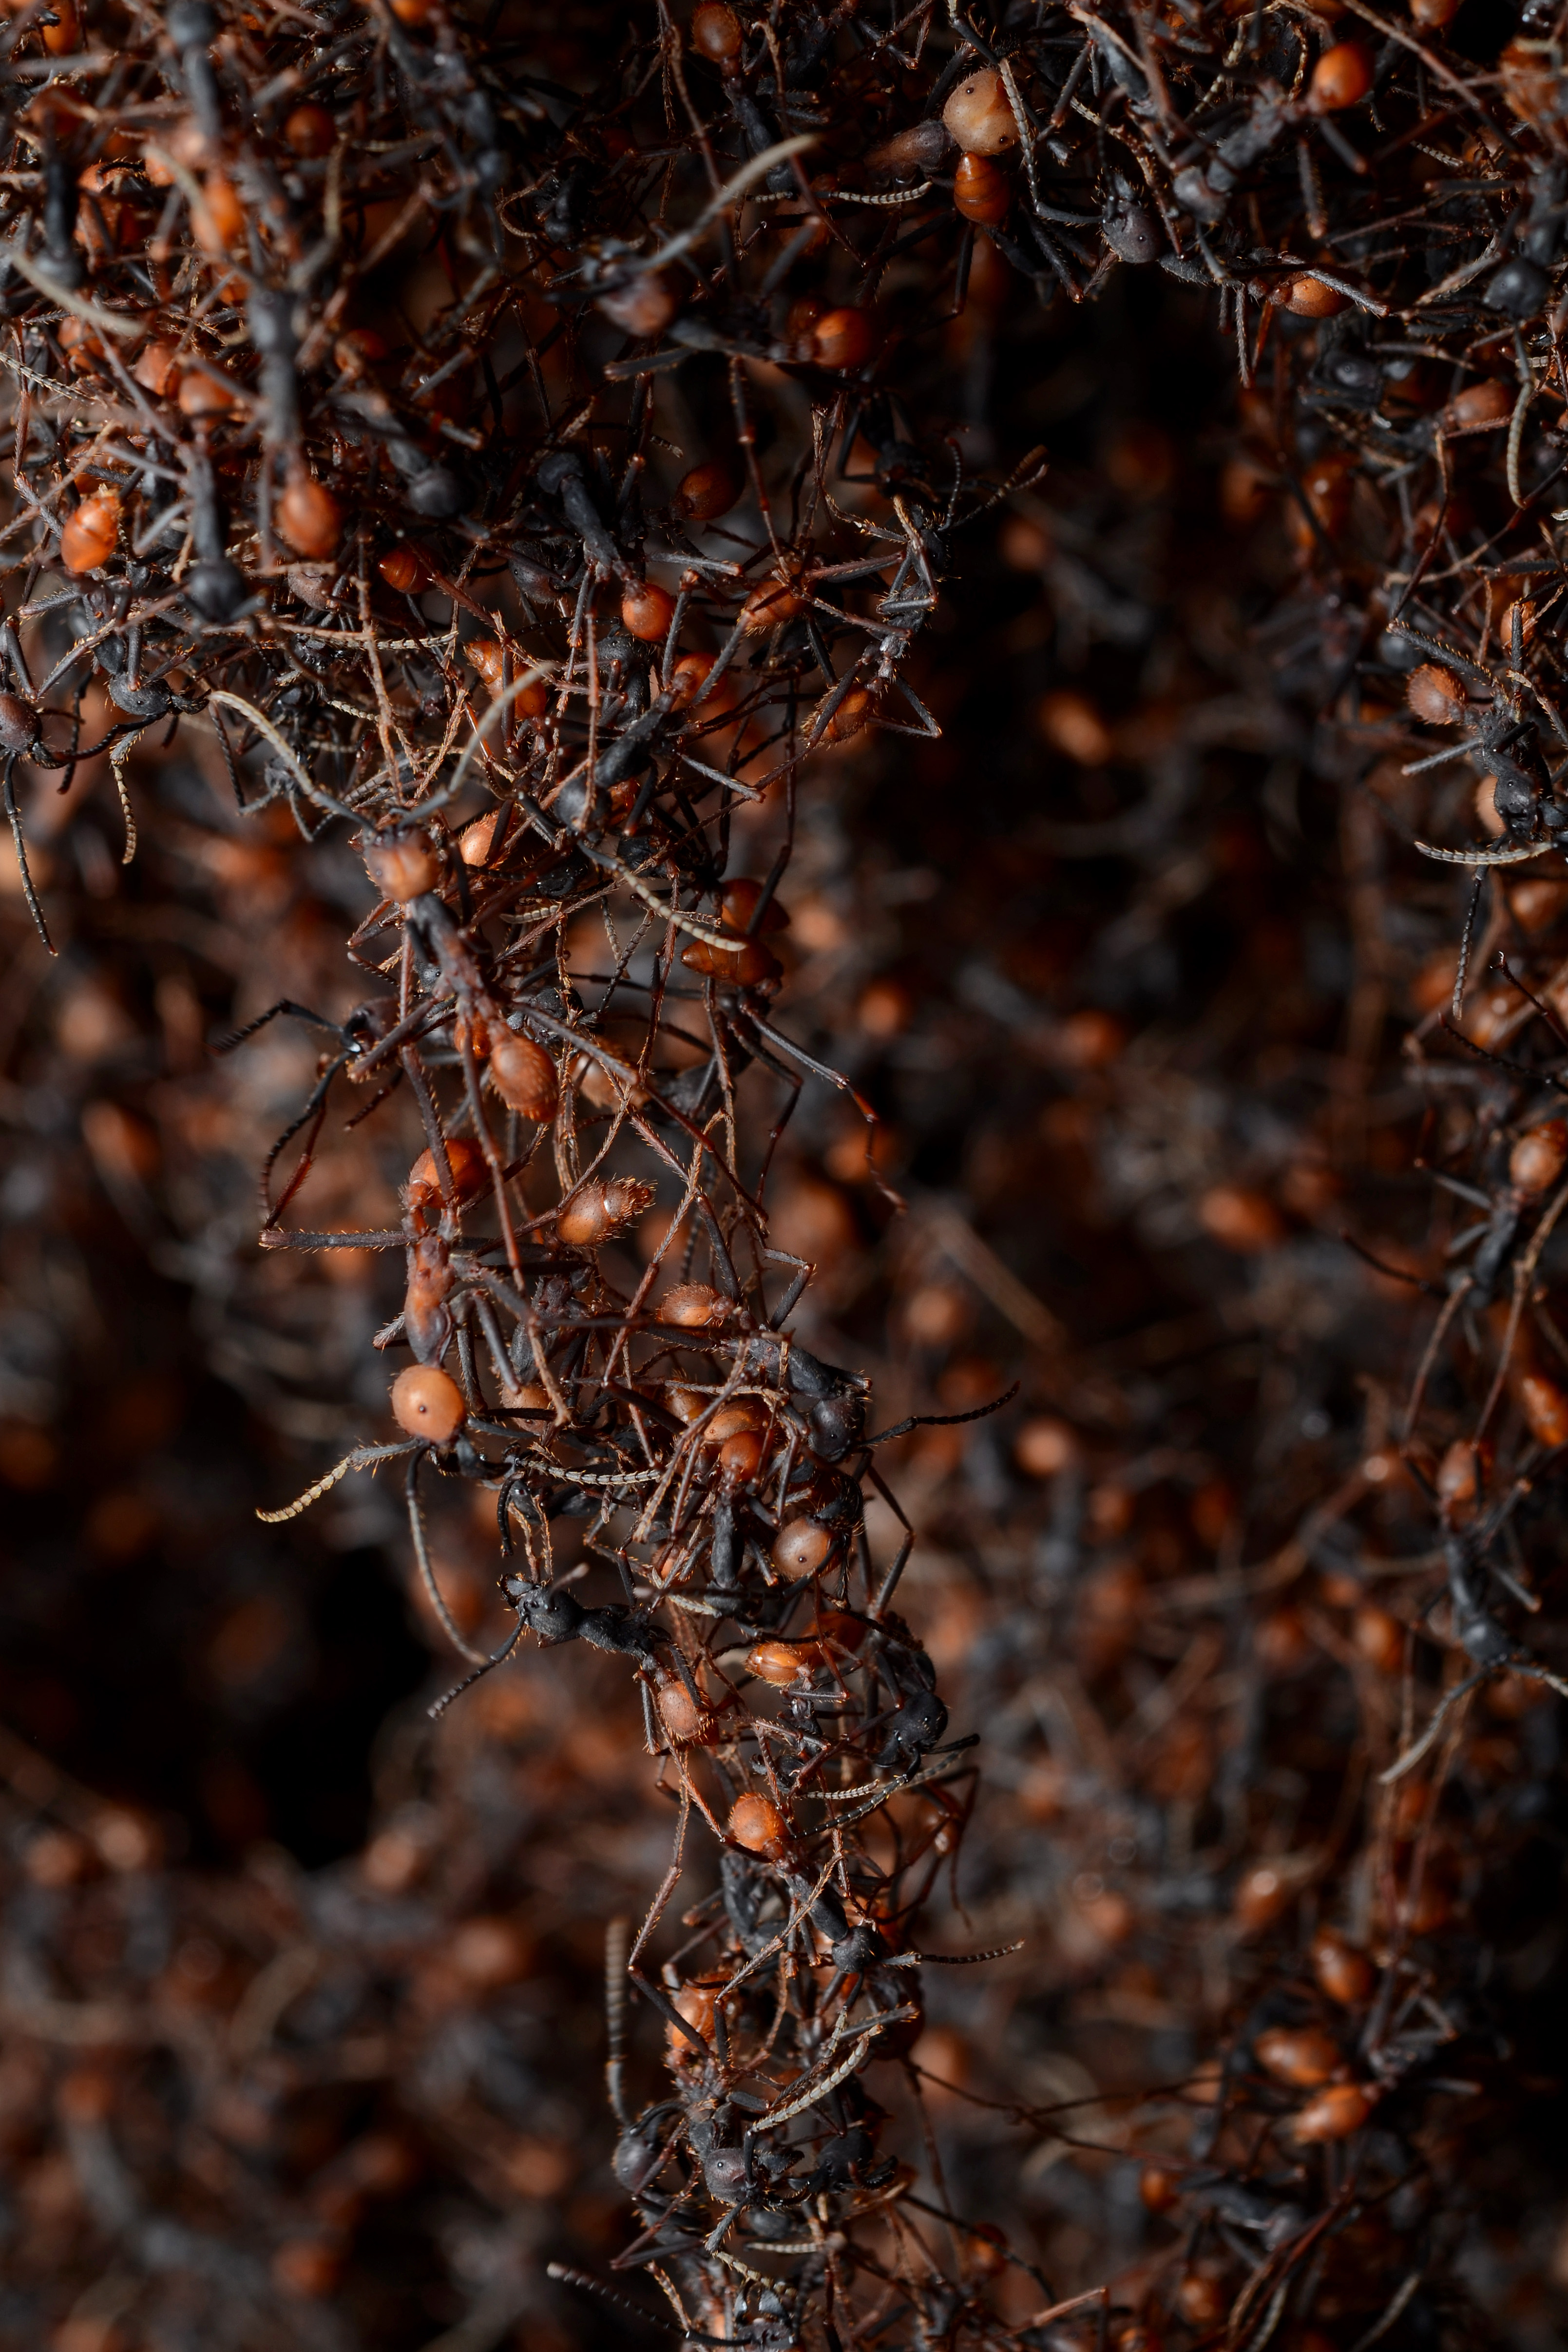
\includegraphics[angle=270,width=\textwidth]{img/ant_bridge}
  \end{column}
  \begin{column}{0.05\textwidth}
    \cite{gallice_2011}
  \end{column}
  \end{columns}
 \caption{
 Example of nested fraternal transitions in individuality where cells (a) unite into multicellular ants (b), which in turn unite into ant colonies (c).
 }
 \label{fig:fraternal}
\end{figure}

\end{alertblock}

\end{block}


\begin{block}{References}
{\tiny\bibliographystyle{abbrv}
\bibliography{bibl}}
\end{block}

\begin{block}{Acknowledgement}
{\footnotesize
Thanks to members of the DEVOLAB, in particular Alexander Lalejini for providing SignalGP graphics.
This research was supported in part by NSF grants DEB-1655715 and DBI-0939454, and by Michigan State University through the computational resources provided by the Institute for Cyber-Enabled Research.
This material is based upon work supported by the National Science Foundation Graduate Research Fellowship under Grant No. DGE-1424871.
Any opinions, findings, and conclusions or recommendations expressed in this material are those of the author(s) and do not necessarily reflect the views of the National Science Foundation.\par
}
\end{block}



%------------------------------------------------

%----------------------------------------------------------------------------------------
%	OBJECTIVES
%----------------------------------------------------------------------------------------


%----------------------------------------------------------------------------------------

\end{column} % End of the first column

\begin{column}{\sepwid}\end{column} % Empty spacer column

\begin{column}{\twocolwid} % Begin a column which is two columns wide (column 2)

%----------------------------------------------------------------------------------------
%	IMPORTANT RESULT
%----------------------------------------------------------------------------------------


\begin{block}{Model System}
\begin{figure}
  \centering
\begin{columns}
\begin{column}{0.25\textwidth}
  \begin{subfigure}[b]{\textwidth}
    
\includegraphics[width=\textwidth,trim={300 300 250 250},clip]{img/lifecycle-1}
    \caption{unicellular group}
    \label{fig:lifecycle-1}
  \end{subfigure}%
\end{column}
\begin{column}{0.05\textwidth}
  \vspace{3ex}
  
\includegraphics[width=\textwidth]{img/arrow}
\end{column}
\begin{column}{0.25\textwidth}
  \begin{subfigure}[b]{\textwidth}
    
\includegraphics[width=\textwidth,trim={300 300 250 250},clip]{img/lifecycle-2}
    \caption{multicellular group}
    \label{fig:lifecycle-2}
  \end{subfigure}%
\end{column}
\begin{column}{0.05\textwidth}
  \vspace{3ex}
  
\includegraphics[width=\textwidth]{img/arrow}
\end{column}
\begin{column}{0.25\textwidth}
  \begin{subfigure}[b]{\textwidth}
    
\includegraphics[width=\textwidth,trim={300 300 250 250},clip]{img/lifecycle-3}
    \caption{multicell w/ propagule}
    \label{fig:lifecycle-3}
  \end{subfigure}%
\end{column}
\begin{column}{0.2\textwidth}
\caption{
Example of nested fraternal transitions of individuality where cells (\ref{fig:cheek_cell}) unite into multicellular ants (\ref{fig:ant}), which in turn unite into ant colonies (\ref{fig:ant_bridge}).
}
\label{fig:fraternal}
\end{column}
\end{columns}
\end{figure}

\vspace{4ex}
\begin{figure}
  \centering
  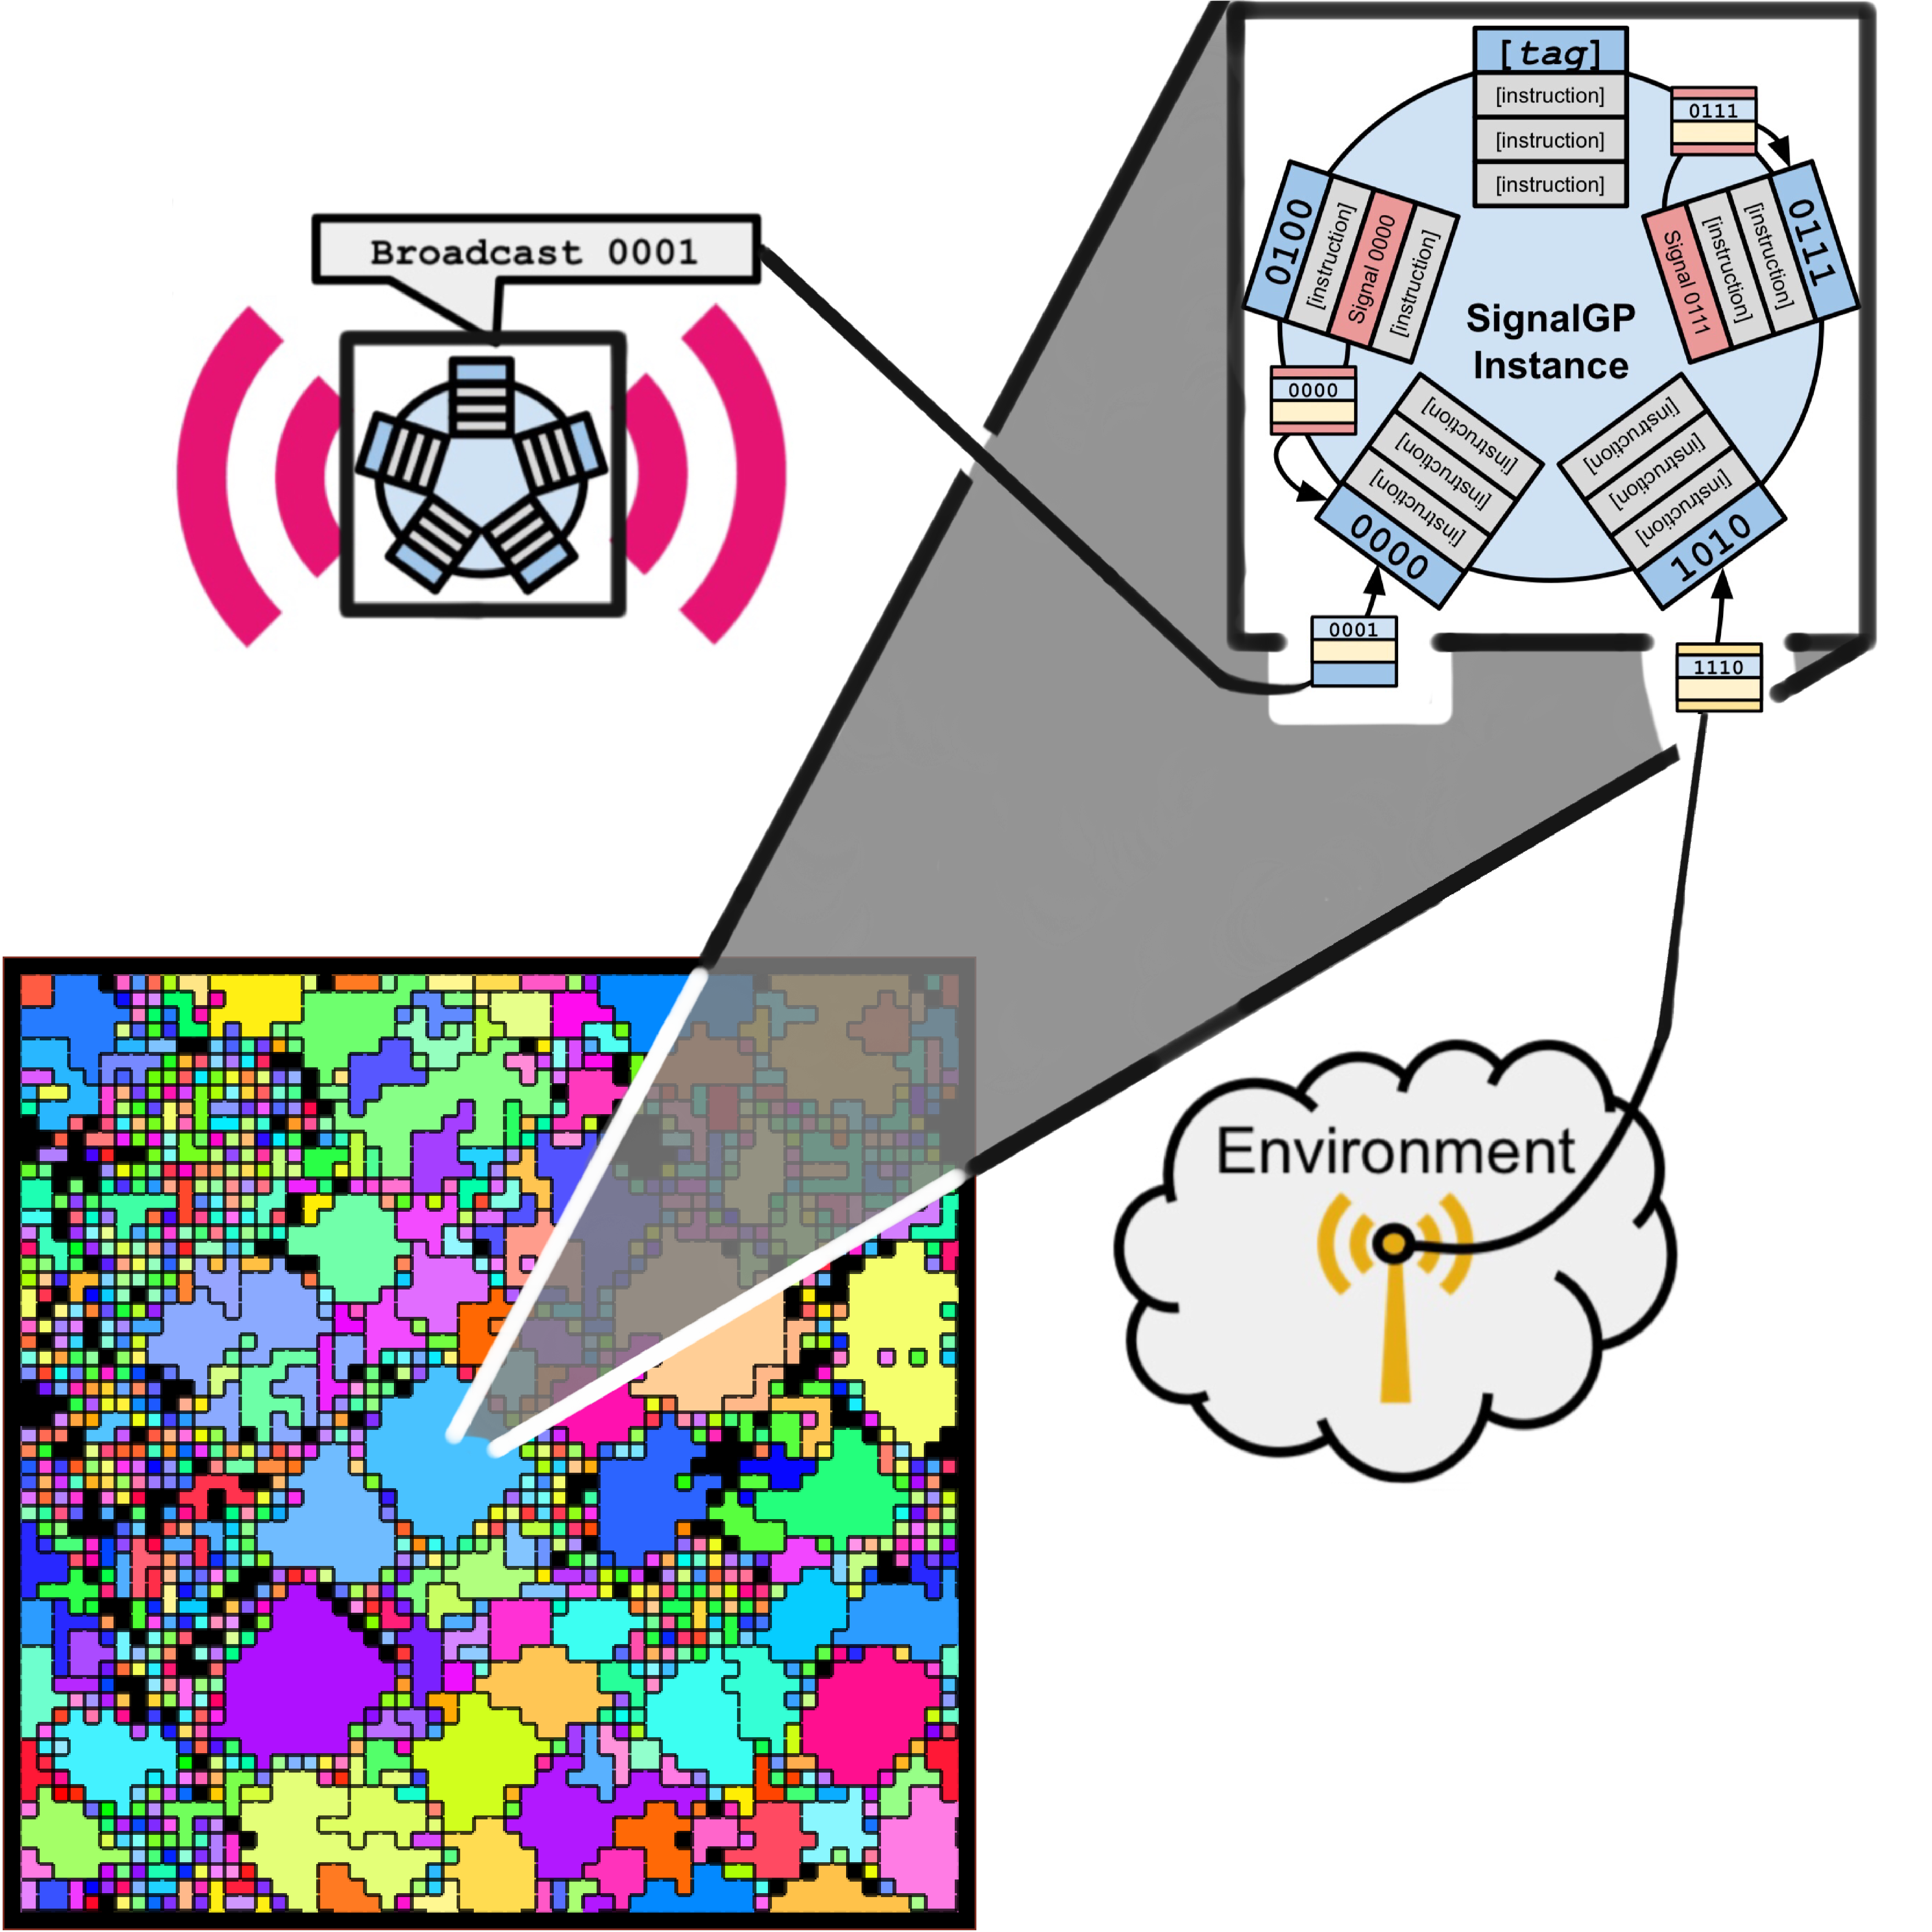
\includegraphics[width=\textwidth]{img/schematic}
  \vspace{-10ex}
  \begin{columns}
  \begin{column}{0.52\textwidth}
  \end{column}
  \begin{column}{0.48\textwidth}
  \caption{
  Experiments track digital cells on a fixed-size toroidal grid (bottom left).
  Resource-collecting group (contiguous same-color clumps) size determines cellular reproduction rate.
  Per-cell resource-collection rate increases with group size up to a threshold group size, where it begins to diminish.
  Heritable SignalGP programs (inset, top right) \cite{lalejini2018evolving} control each cell, deciding when to reproduce, where to place daughter cell, whether to grow the parent's group or start a new group, apoptosis, resource-sharing, and intercellular communication.
  }
  \label{fig:model}
  \end{column}
  \end{columns}
\end{figure}

\end{block}



%----------------------------------------------------------------------------------------
\vspace{-6ex}
\begin{columns}[t,totalwidth=\twocolwid] % Split up the two columns wide column again

\begin{column}{\onecolwid} % The first column within column 2 (column 2.1)


%----------------------------------------------------------------------------------------

\end{column} % End of column 2.1

\begin{column}{\onecolwid} % The second column within column 2 (column 2.2)


\end{column} % End of column 2.2

\end{columns} % End of the split of column 2

\end{column} % End of the second column

\begin{column}{\sepwid}\end{column} % Empty spacer column

\begin{column}{\onecolwid} % The third column

\begin{block}{Preliminary Results}
\begin{alertblock}{Resource Sharing}
  \begin{figure}
  \begin{columns}
  \begin{column}{0.7\textwidth}
  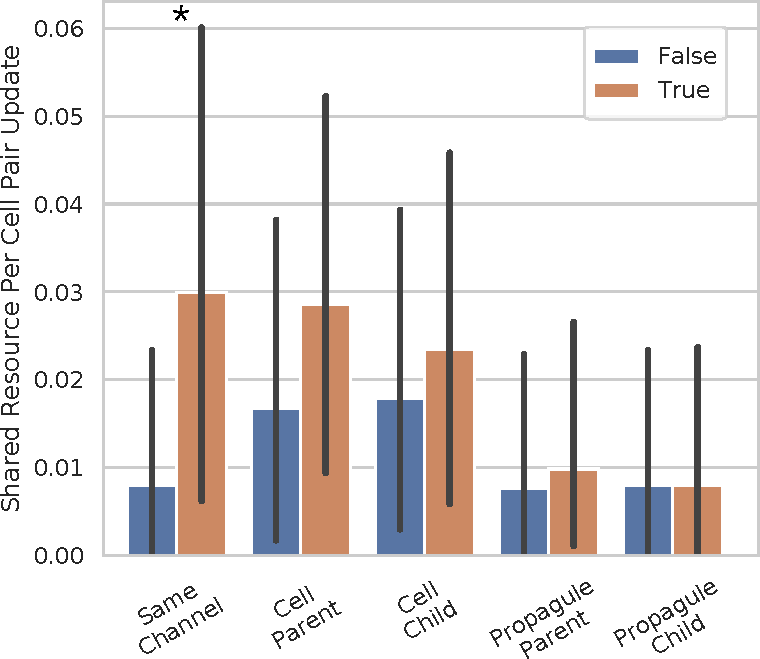
\includegraphics[width=\textwidth]{img/channelsense-yes__nlev-two+title=resource_contributed+ext=}
  \end{column}
  \begin{column}{0.3\textwidth}
  \caption{
  TODO
  }
  \label{fig:sharing}
  \end{column}
  \end{columns}
\end{figure}

\end{alertblock}
\begin{alertblock}{Reproductive Differentiation}
  \begin{figure}
  \begin{columns}
  \begin{column}{0.75\textwidth}
  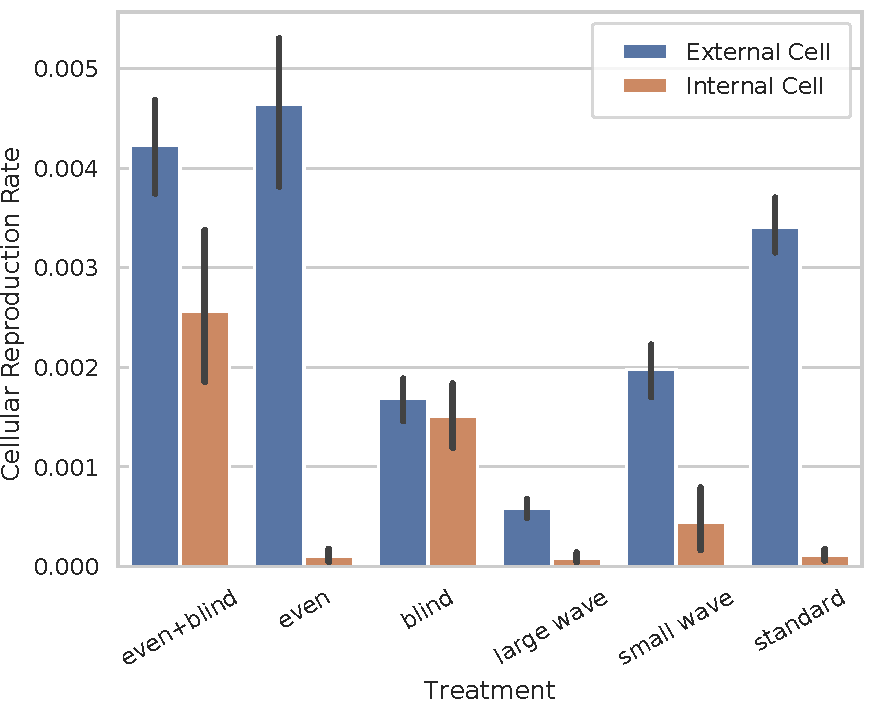
\includegraphics[width=\textwidth]{img/title=reproductive_labor_surrounded+ext=}
  \end{column}
  \begin{column}{0.25\textwidth}
  \caption{
  Evolved phenotypes delegate reproduction to the exterior of resource-collection groups.
  }
  \label{fig:differentiation}
  \end{column}
  \end{columns}
\end{figure}

\end{alertblock}
\begin{alertblock}{Propagule Endowment}
  \begin{figure}
\begin{columns}
\begin{column}{0.75\textwidth}
  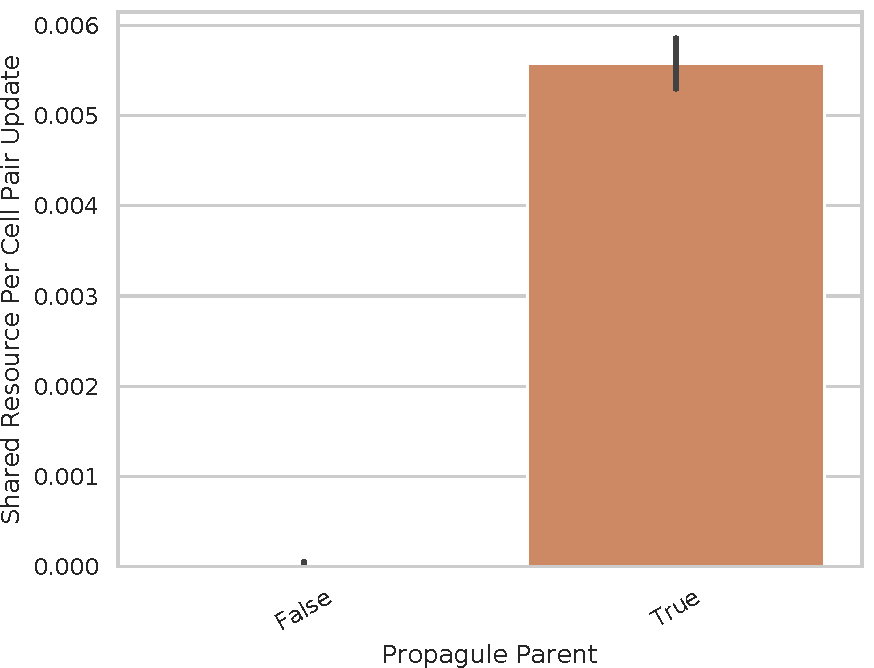
\includegraphics[width=\textwidth]{img/treat=resource-wave__channelsense-yes__nlev-two+seed=1018+title=propagule_parent_resource_contributed+ext=}
\end{column}
\begin{column}{0.25\textwidth}
  \caption{
  In some replicates, cell groups evolve to share resource with propagule groups.
  }
  \label{fig:endowment}
\end{column}
\end{columns}
\end{figure}

\end{alertblock}
\end{block}


\begin{block}{Next Steps}
\vspace{-1ex}
{\small
\begin{itemize}
\item TODO
\end{itemize}
}
\vspace{-1ex}
\end{block}


\end{column} % End of the third column

\end{columns} % End of all the columns in the poster

\end{frame} % End of the enclosing frame

\end{document}
